\documentclass[12pt,a4paper]{article}
\usepackage[utf8]{inputenc}
\usepackage[T1]{fontenc}
\usepackage[spanish]{babel}
\usepackage{amsmath}
\usepackage{amsfonts}
\usepackage{amssymb}
\usepackage{comment}
\usepackage{float} 
\usepackage{graphicx}
\usepackage[left=3.00cm, right=3.00cm, top=2.50cm, bottom=2.50cm]{geometry}
\author{Caamiña Quineros, Daniela Beatriz\\ \and Yapura, Cristian Alejandro}
\title{Proyecto final}
\graphicspath{ {imagenes/} }

\newcommand{\grad}{$^{\circ}$}
\begin{document}
	\maketitle
	\newpage
	\thanks{Agradecimiento}
	\newpage
	\tableofcontents
	\newpage
	\listoffigures
	\newpage

	\section{Introducción}
	Actualmente en el Laboratorio de Automatización y Control de la Universidad, se cursan distintas materias en las cuales se necesitan herramientas para realizar diversas prácticas, con el fin de afianzar los conocimientos que se adquieren a lo largo del año.
\\

Para llevar a cabo estas actividades con varias etapas, se requiere demasiado tiempo en realizar pruebas sobre un esquema complejo, es decir con varios elementos, ya que se necesita armar un prototipo de banco de prueba cada vez que sea necesario. Por ejemplo, realizar la conexión de un PLC, variador de frecuencia y un motor puede ser una tarea repetitiva que se busca suprimir. 

\newpage

	\section{Objetivo}
	Generar un lazo de control que tenga como entrada la velocidad de referencia, y que contemple las perturbaciones externas del sistema en el cálculo de la velocidad de salida que se utilizará como lazo de realimentación. 
Adaptar la acción de control que ingresa al variador de velocidad (adquirido por el Laboratorio de Fluidos) para alimentar al motor y dejar en desuso el banco de resistencias que se utiliza.
Además, realizar una interfaz gráfica para un mejor manejo y control del sistema.

\begin{figure}[htb]
	\centering
	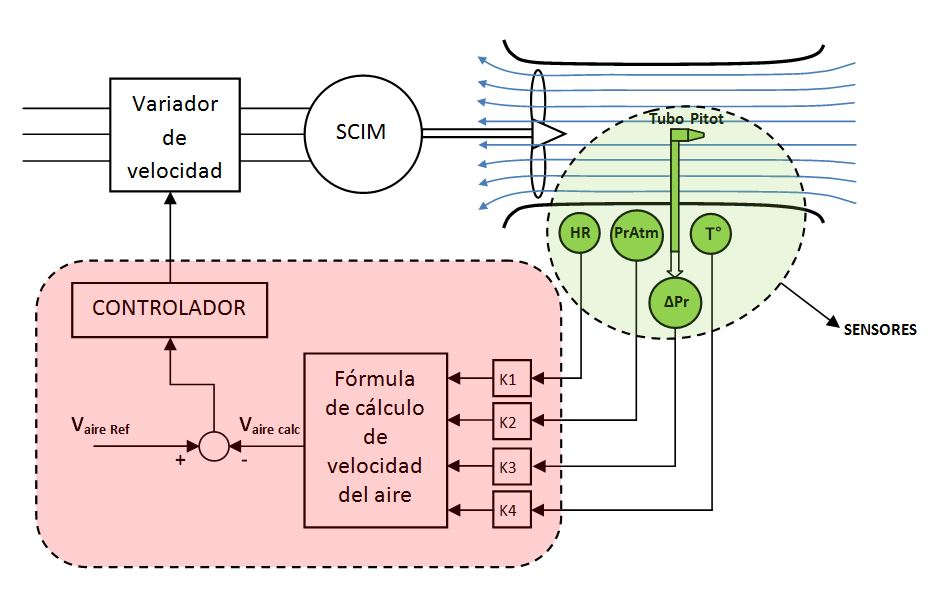
\includegraphics[scale=0.35]{diagr.jpg}
	\caption{Diagrama}
	\label{fig:diagr}
	\end{figure}

	\section{Palabras claves}
	\input{secciones/Palabras}

	\section{Tunel}
	\subsection{¿Qué es?}
Un túnel de viento es una herramienta que puede tener dos fines hoy en día, ya sea para un uso recreativo o propósito científico.
Como uso científico se utiliza para observar los efectos del movimiento de aire al rededor de objetos sólidos, como tambien para la calibración de anemómetros.
\begin{figure}[htb]
	\centering
	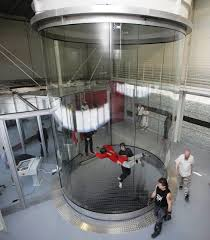
\includegraphics[scale=0.35]{tvert1.jpg}
	\caption{Tunel uso recreativo}
	\label{fig:tunelRec}
	\end{figure}
Los túneles de viento se pueden clasificar en túneles abiertos o cerrados y a su vez pueden ser verticales u horizontales.

\subsection{Historia del Túnel UNPSJB}
\footnote{http://www.ing.unp.edu.ar/mecanica/Paginas/Tunel.htm} 
	El túnel aerodinámico del Laboratorio de Mecánica de Fluidos (LMF) de la Facultad de Ingeniería de la Universidad Nacional de la Patagonia San Juan Bosco (UNPSJB) es un circuito abierto (tipo Eiffel) con cámara de ensayos cerrada. Puede clasificarse como un túnel “pequeño de baja velocidad”, con una longitud total de 11m, una velocidad máxima de 18 m/s y una cámara de ensayos con un área de 0,8m2.
	\\
	La entrada del túnel cuenta con canalizadores, comúnmente denominados "panal de abejas", que favorecen la formación de un flujo uniforme y homogéneo propiciando mejores resultados en los experimentos.
	\\
	La cámara de ensayos es vidriada para poder observar con claridad el flujo y está incorporada en un módulo extraíble del túnel, lo cual permite fácil acceso para el armado de los distintos objetos a ensayar.
	\\
	La variación de la velocidad del aire dentro de la cámara se consigue por dos vías: modificando la velocidad del motor para lograr una aproximación, y mediante la apertura de compuertas ubicadas entre el rodete y la zona de ensayo, para el ajuste fino. La toma aire desde el exterior a través de las compuertas actúa como by-pass, modificando el flujo principal del túnel y controlando su velocidad.
	\\
	Los distintos ensayos que se realizan en el túnel son:
	\\
	- Determinación de coeficientes de resistencia y sustentación de distintos cuerpos y perfiles aerodinámicos.
	- Determinación de distribución de presiones a través de diferentes objetos como perfiles aerodinámicos, edificios, puentes, automóviles, etc.
	- Visualización con humo del flujo a través de distintos obstáculos.
	- Estudio del comportamiento dinámico de generadores eólicos.
	- Calibración de anemómetros. 

	\begin{figure}[htb]
		\centering
		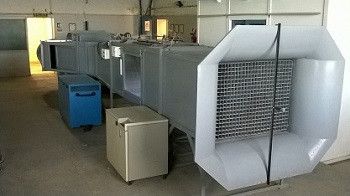
\includegraphics[scale=0.35]{tunel_unpsjb.JPG}
		\caption{Tunel UNPSJB}
		\label{fig:tunelUni}
		\end{figure}	

	\section{Motor}
	\subsection{Especificaciones}

	El motor (Figura \ref{fig:motor}) asincrónico que se utiliza es de la marca \textbf{Altium} perteneciente a la firma \textbf{Schneider Electric}. Las especificaciones se muestran a continuación \\
	\paragraph*{Altium Eff2}
	\begin{itemize}
		\item 	Tipo: TE2A90SP2
		\item   Tensión nominal: 220/380 V
		\item 	Corriente nominal: 5.97 A 
		\item	Frecuencia nominal:  50 Hz.
		\item 	Potencia: 1.5kW / 2 HP
		\item 	Fases: 3
		\item   Factor de Potencia: 0.84
	\end{itemize}
	\newpage
	\begin{figure}[h!]
		\centering
		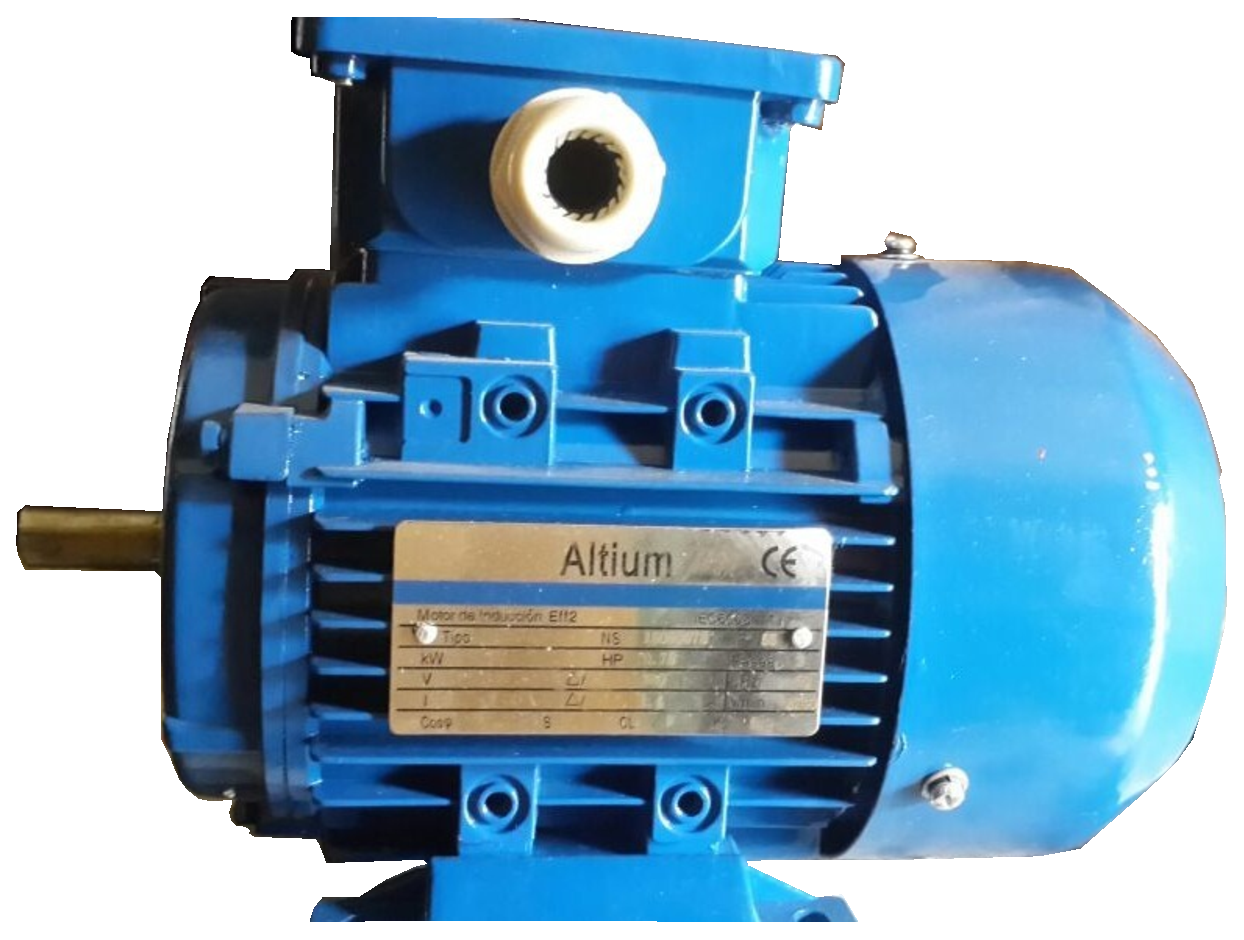
\includegraphics[scale=0.4]{motor.eps}
		\caption{Motor Altium}
		\label{fig:motor}
	\end{figure}
	\newpage

	\section{Variador}
	\subsection{Especificaciones}
El variador de velocidad que se utilizó pertenece a la marca \textbf{Schneider Electric} (Figura \ref{fig:variador}) que posee las siguientes características. \\
	\paragraph*{Altivar 312}
	\begin{itemize}
		\item 	Modelo: ATV312HU15N4
		\item   Tensión: 380-500 V
		\item 	Frecuencia: 50/60 Hz
		\item 	Potencia: 1.5kW / 2 HP
		\item 	Fases: 3
	\end{itemize}

	\begin{figure}[h!]
		\centering
		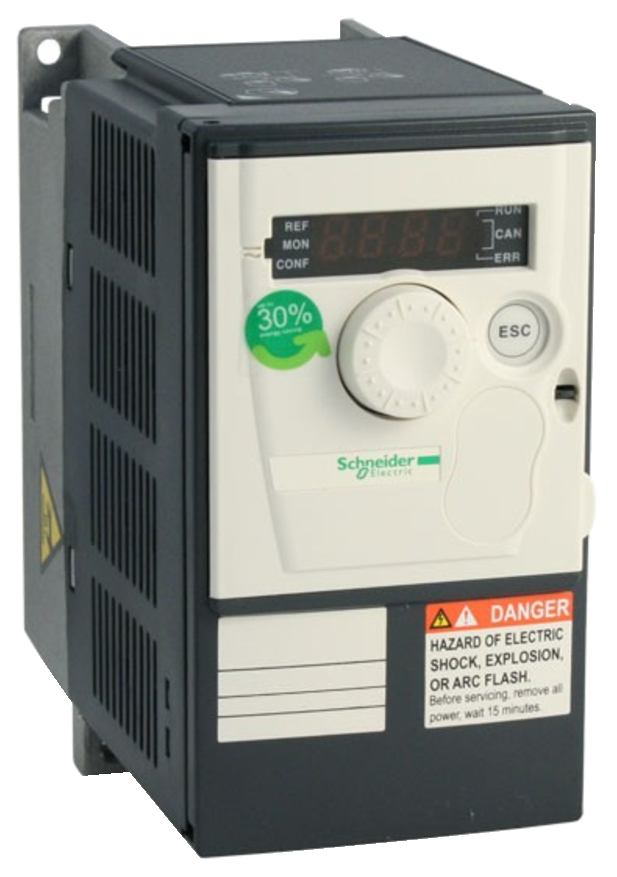
\includegraphics[scale=0.4]{variador.eps}
		\caption{Variador de velocidad Altivar 312}
		\label{fig:variador}
	\end{figure}


	\subsection{Configuración de parámetros primarios}
	Para realizar la configuración del motor se utilizó el software SoMove. Se descargó la ultima versión desde la página oficial de Schneider\footnote{\url{https://www.se.com/ar/es/product-range-presentation/2714-somove/}} y luego, la librería DTM correspondiente al variador a utilizar\footnote{\url{https://www.se.com/ar/es/download/document/Altivar_DTM_Library/}}. 
	\\
	Una vez realizado esto se procedió a generar un nuevo proyecto eligiendo las opciones correctas del variador.
	
	
	\newpage


	


	
	\section{Cálculo de la densidad del aire}
		
	\part{Desarrollo}
	\section{Primeras pruebas}
	\subsection{Sensores}
	\subsubsection{SHT31-SHT21}
	SHT31 es un sensor digital de temperatura y humedad relativa. Posee protocolo I2C.
	\paragraph*{Especificaciones}
	\begin{itemize}
		\item   Voltaje de operación: 2.4 V a 5.5 V.
		\item	Rango de temperatura: -40\grad C a 12\grad C.
		\item   Resolución de temperatura: 0.015\grad C
		\item	Precisión de temperatura: 0.2\grad C 
		\item	Rango de humedad: 0 a 100\% RH
		\item   Resolución HR: 0.01 \% RH
		\item   Precisión HR: 2\% RH
		\item Frecuencia de muestreo: 157 Hz.
	\end{itemize}
		\begin{figure}[htb]
	\centering
	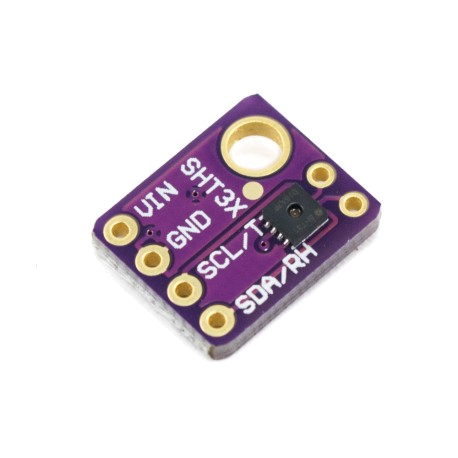
\includegraphics[scale=0.35]{SHT31.png}
	\caption{Placa SHT31}
	\label{fig:SHT31}
		\end{figure}
	
	\subsubsection{BME280}
	BME280 es un dispositivo que mide presión atmosférica, temperatura y humedad relativa, con gran precisión, bajo consumo y compacto. Utiliza protocolo I2C para su comunicación.
		\paragraph*{Especificaciones}
		\begin{itemize}
		\item   Voltaje de operación: 1.8 V a 3.3 V.
		\item	Rango de temperatura: -40\grad C a 85\grad C.
		\item   Resolución de temperatura: 0.01\grad C
		\item	Precisión de temperatura: 1\grad C 
		\item	Rango de humedad: 0 a 100\% RH
		\item   Precisión HR: 3\% RH
		\item Rango de Presión: 300 a 1100 hPa (0.3-1.1bar)
		\item Resolución de presión: 0.16 Pa
	\end{itemize}
	
		\begin{figure}[htb]
		\centering
		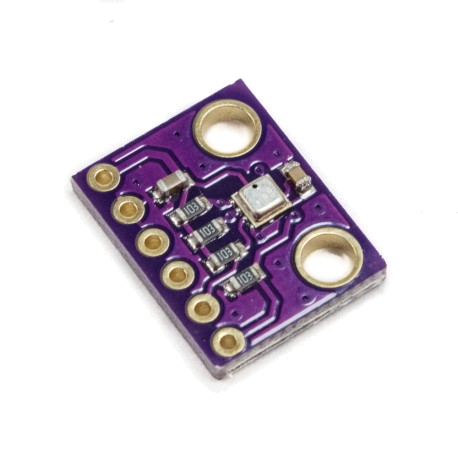
\includegraphics[scale=0.35]{bme280.png}
		\caption{Placa BME280}
		\label{fig:BME280}
		\end{figure}
	
	\subsubsection{MPX7002}
	
	\subsection{Matlab}
	\subsection{Arduino}
	\section{Lazo de control}
	\subsection{Comunicación del variador de Velocidad}
	\subsubsection{0-10V}
	\subsubsection{4-20mA}
	\subsubsection{MODBUS}
	\section{Microcontrolador}
	\subsection{Arduino- CIAA}

\newpage

 \begin{comment}
\bibliography{biblio}
https://mauricioanderson.com/curso-latex-referencias-bibliografia-bibtex/ ver esto
\begin{thebibliography}{0}
	\bibitem{TunelUNPSJB} http://www.ing.unp.edu.ar/mecanica/Paginas/Tunel.htm.
	\bibitem{Luckie2010} Matthew Luckie. CScamper: a scalable, extensible packet 
	prober for active measurement of the internet, 2010.
\end{thebibliography}
\newpage
\part{Anexos}

\end{comment}



\end{document}